% Adjust these for the path of the theme and its graphics, relative to this file
%\usepackage{beamerthemeFalmouthGamesAcademy}
\usepackage{../../beamerthemeFalmouthGamesAcademy}
\graphicspath{ {../../} }

% Default language for code listings
\lstset{language=C++,
        morekeywords={each,in,nullptr}
}

\begin{document}
\title{Transition to C++ III}   
\subtitle{COMP110: Principles of Computing}

\frame{\titlepage} 

\begin{frame}{Learning outcomes}
    In this session you will learn how to...
    \begin{itemize}
        \item Define your own \textbf{classes} in C++
        \item Use \textbf{pointers}, and allocate objects on the \textbf{heap}
        \item Use \textbf{typecasting} to convert values from one type to another
        \item Use the \textbf{CImg} library to write basic GUI applications and image processing algorithms
    \end{itemize}
\end{frame}

\part{Object-oriented programming in C++}
\frame{\partpage}

\begin{frame}[fragile]{OOP refresher}
    \begin{itemize}
        \item A \textbf{class} is a collection of \textbf{fields} (data) and \textbf{methods} (functions)
        \item Fields and methods may be \textbf{public} (accessible everywhere), \textbf{protected} (accessible in the class and classes that inherit from it) or \textbf{private} (accessible in the class only)
        \item Classes may \textbf{inherit} fields and methods from other classes
        \item Subclasses may \textbf{override} methods which they inherit --- this gives rise to \textbf{polymorphism}
    \end{itemize}
\end{frame}

\begin{frame}[fragile]{Class declarations}
    \begin{lstlisting}
class MyClass
{
public:
    void doMethod(int x)
    {
        std::cout << x << std::endl;
    }

private:
    int field = 7;
};
    \end{lstlisting}
\end{frame}

\begin{frame}[fragile]{Fields and methods}
    \begin{itemize}
        \item Fields and methods are declared in the class declaration, just like variables and functions
        \item Class declaration is split into sections by access type (\textbf{public}, \textbf{protected}, \textbf{private})
    \end{itemize}
\end{frame}

\begin{frame}[fragile]{Overloading}
    \begin{itemize}
        \item Functions and methods can be defined with the \textbf{same name} but \textbf{different parameters}
    \end{itemize}
    \begin{lstlisting}
    double getVectorLength(double x, double y)
    {
        return sqrt(x * x + y * y);
    }

    double getVectorLength(Vector v)
    {
        return sqrt(v.x * v.x + v.y * v.y);
    }
    \end{lstlisting}
\end{frame}

\begin{frame}[fragile]{Constructors and destructors}
    \begin{itemize}
        \item The \textbf{constructor} is executed when the class is instantiated
        \item The \textbf{destructor} is executed when the instance is freed
    \end{itemize}
	\begin{lstlisting}
class MyClass
{
public:
    MyClass()
    {
    }
    
    ~MyClass()
    {
    }
};
	\end{lstlisting}
\end{frame}

\begin{frame}[fragile]{Constructors}
    \begin{itemize}
        \item The constructor name matches the class name
        \item Constructors can take parameters
        \item The constructor can be overloaded, i.e.\ can have several constructors with different parameters
    \end{itemize}
	\begin{lstlisting}
class MyClass
{
public:
    // Parameterless constructor
    MyClass() { }
    
    // Constructor with parameters
    MyClass(int x, double y) { }
};
	\end{lstlisting}
\end{frame}

\begin{frame}[fragile]{Destructors}
    \begin{itemize}
        \item The destructor name is the class name prefixed with $\sim$ (tilde)
        \item Destructors \textbf{cannot} take parameters
    \end{itemize}
\end{frame}

\begin{frame}[fragile]{Modular program design}
    \begin{itemize}
        \item Method \textbf{declarations} go in the class declaration
        \item Method \textbf{definitions} look like function definitions,
            with the function name replaced with \lstinline{ClassName::methodName}
        \item Method definitions can also go inline into the class declaration
        \begin{itemize}
            \item Best used for short (1 or 2 line) methods
        \end{itemize}
        \item Good practice: Put class declaration in \texttt{ClassName.h}, and method definitions in \texttt{ClassName.cpp}
    \end{itemize}
\end{frame}

\begin{frame}[fragile]{Example: Circle.h}
    \begin{lstlisting}
#pragma once

class Circle
{
public:
    Circle(double radius);
    
    double getArea();

private:
    double radius;
};
    \end{lstlisting}
\end{frame}

\begin{frame}[fragile]{Example: Circle.cpp}
    \begin{lstlisting}
#include "stdafx.h"
#include "Circle.h"

Circle::Circle(double radius)
    : radius(radius)
{
}

double Circle::getArea()
{
    return M_PI * radius * radius;
}
    \end{lstlisting}
\end{frame}

\begin{frame}[fragile]{Inheritance}
    \begin{lstlisting}
class Shape
{
public:
    virtual double getArea();
};

class Circle : Shape
{
public:
    virtual double getArea()
    {
        return M_PI * radius * radius;
    }
};
    \end{lstlisting}
    \begin{itemize}
        \item Methods to be overridden must be marked \textbf{virtual}
    \end{itemize}
\end{frame}

\begin{frame}[fragile]{Pure virtual methods}
    \begin{itemize}
        \item \textbf{Abstract classes} should never be instantiated --- they only exist to serve as a base class
        \item \textbf{Abstract methods} are not defined in the base class, and must be overridden in the subclass
        \item In C++, abstract methods are called \textbf{pure virtual}
        \item Having at least one pure virtual method \textbf{automatically} makes the class abstract
    \end{itemize}
    \begin{lstlisting}
class Shape
{
public:
    virtual double getArea() = 0;
};
    \end{lstlisting}
\end{frame}

\begin{frame}[fragile]{Instantiation}
    \begin{itemize}
        \item To instantiate with a \textbf{parameterless constructor}, just declare a variable
    \end{itemize}
    \begin{lstlisting}
MyClass myInstance;
    \end{lstlisting}
    \begin{itemize}
        \item To instantiate with a \textbf{constructor with parameters}, add the parameters in parentheses
    \end{itemize}
    \begin{lstlisting}
MyClass myInstance(27);
    \end{lstlisting}
    \begin{itemize}
        \item This allocates the instance on the \textbf{stack}
        \item The instance is destroyed (and the destructor is called) when the variable goes \textbf{out of scope}
    \end{itemize}
\end{frame}


\part{Arrays and pointers}
\frame{\partpage}

\begin{frame}[fragile]{Arrays in C++}
    \begin{itemize}
        \item An \textbf{array} is a fixed-length sequence of elements of a particular type
        \item Not to be confused with a \textbf{vector}, which is a variable length sequence
    \end{itemize}
    \begin{lstlisting}
// Declare a 5-element array with initial values
int myArray[] = { 1, 3, 5, 7, 9 };

// Declare a 10-element array without specifying initial values
int myOtherArray[10];
    \end{lstlisting}
\end{frame}

\begin{frame}[fragile]{Arrays in memory}
    \begin{center}
        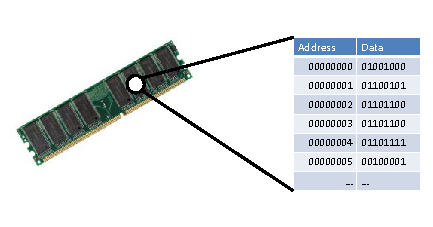
\includegraphics[width=0.6\textwidth]{memory.pdf}
    \end{center}
    \begin{itemize}
        \item An array is a contiguous block of memory
        \item E.g.\ an \lstinline{int} is 4 bytes (32 bits), so an array of 10 \lstinline{int}s is $10 \times 4 = 40$ bytes
        \item The size of the array is \textbf{fixed}: a 10 element array holds exactly 10 elements, forever
    \end{itemize}
\end{frame}

\begin{frame}[fragile]{Index out of range}
    This Python code will give a ``list index out of range'' exception
    \begin{lstlisting}[language=Python]
myList = [1, 3, 5, 7, 9]
print myList[5]
    \end{lstlisting}
    
    This C++ code will give a ``vector subscript out of range'' exception
    \begin{lstlisting}
std::vector<int> myVector = {1, 3, 5, 7, 9};
std::cout << myVector[5] << std::endl;
    \end{lstlisting}
    
    This C++ code will print some arbitrary number
    \begin{lstlisting}
int myArray[] = { 1, 3, 5, 7, 9 };
std::cout << myArray[5] << std::endl;
    \end{lstlisting}
\end{frame}

\begin{frame}[fragile]{Index out of range}
    \begin{itemize}
        \item C++ does not check array indices
        \item It is easy to accidentally read or write past the end of the array, and doing so will cause
            hard-to-fix bugs
        \item \lstinline{myArray} is a 5-element array of \lstinline{int}s, i.e.\ a block of $5 \times 4 = 20$ bytes
        \item If \lstinline{myArray} starts at memory address $1000$, then \lstinline{myArray[i]} is at address
            $1000 + 4 \times i$
        \item \lstinline{myArray[5]} is whatever happens to be at memory address $1000 + 4 \times 5 = 1020$ ---
            could be unallocated memory, could be another variable, could be part of another array,
            could even be part of the machine code being executed
    \end{itemize}
\end{frame}

\begin{frame}[fragile]{Array size must be a compile-time constant}
    \begin{lstlisting}
double a[10];            // OK

const int size = 10;
double b[size];          // OK
double c[2 * size + 7];  // OK

int varSize = 10;
double d[varSize];       // Error
    \end{lstlisting}
\end{frame}

\begin{frame}[fragile]{Dynamic allocation}
    \begin{itemize}
        \item If the size of the array is not known in advance, it can be allocated at runtime
            using the \lstinline{new} keyword
    \end{itemize}
    \begin{lstlisting}
int n = readNumberFromConsole();
int* myArray = new int[n];
    \end{lstlisting}
    \begin{itemize}
        \item Technically \lstinline{myArray} is no longer an array, it's a \textbf{pointer}
        \item \lstinline{int*} is the type ``pointer to an \lstinline{int}''
        \item Pointers can (mostly) be used as if they were arrays
    \end{itemize}
\end{frame}

\begin{frame}[fragile]{Stack and heap}
    \begin{itemize}
        \item Variables and static arrays are stored on the \textbf{stack}
        \begin{itemize}
            \item Stack items are automatically freed when they go out of scope
        \end{itemize}
        \item Anything created with \lstinline{new} is stored on the \textbf{heap}
        \begin{itemize}
            \item Heap items must be freed with \lstinline{delete} when they are finished with
            \item Forgetting to free them is a \textbf{memory leak}
        \end{itemize}
    \end{itemize}
\end{frame}

\begin{frame}[fragile]{Strings revisited}
    \begin{itemize}
        \item \lstinline{std::string} is the high-level string class
        \item The low-level way of storing strings is as an array of \lstinline{char}s
    \end{itemize}
    \begin{lstlisting}
char greeting[] = "Hello, world!";
    \end{lstlisting}
    \begin{itemize}
        \item Strings are \textbf{null terminated} --- they end with ASCII character 0
    \end{itemize}
\end{frame}

\begin{frame}[fragile]{String literals}
    \begin{lstlisting}
std::string greeting = "Hello, world!";
    \end{lstlisting}
    \begin{itemize}
        \item The thing on the right hand side is actually a \lstinline{char} array, not a \lstinline{std::string}
        \item The assignment operator knows how to convert from \lstinline{char[]} to \lstinline{std::string}
    \end{itemize}
\end{frame}

%\begin{frame}[fragile]{Pointers}
%    \begin{itemize}
%        \item C++ allows us to store and manipulate \textbf{pointers} a.k.a.\ memory addresses
%    \end{itemize}
%    \begin{lstlisting}
%int myVar = 7;
%int* myPointer = &myVar;
%*myPointer = 12;
%    \end{lstlisting}
%    \begin{itemize}
%        \item \lstinline{int*} is a type: pointer to int
%        \item \lstinline{&} is the \textbf{address-of} operator:
%            read \lstinline{&myVar} as ``a pointer to \lstinline{myVar}''
%        \item \lstinline{*} on line 3 is the \textbf{dereference} operator:
%            read \lstinline{*myPointer} as ``the value pointed to by \lstinline{myPointer}''
%    \end{itemize}
%\end{frame}

\begin{frame}[fragile]{2-dimensional arrays}
    Array of arrays approach:
    \begin{lstlisting}
const int width = 8, height = 8;
int grid[width][height];
grid[x][y] = 7;
    \end{lstlisting}
    Flat array approach:
    \begin{lstlisting}
const int width = 8, height = 8;
int grid[width * height];
grid[x + y * width] = 7;
    \end{lstlisting}
\end{frame}


\part{Typecasting}
\frame{\partpage}

\begin{frame}[fragile]{Type conversion}
    \begin{itemize}
        \item Some type conversions happen automatically
    \end{itemize}
    \begin{lstlisting}
int a = 27;
double b = a;
    \end{lstlisting}
\end{frame}

\part{The CImg library}
\frame{\partpage}

\begin{frame}[fragile]{Arrays in C++}
    \begin{itemize}
        \item An \textbf{array} is a fixed-length sequence of elements of a particular type \pause
        \item Not to be confused with a \textbf{vector}, which is a variable length sequence \pause
    \end{itemize}
    \begin{lstlisting}
// Declare a 5-element array with initial values
int myArray[] = { 1, 3, 5, 7, 9 };

// Declare a 10-element array without specifying initial values
int myOtherArray[10];
    \end{lstlisting}
\end{frame}


% -------------------------------------------------------

%\part{The compiler}
%\frame{\partpage}
%
%\begin{frame}
%	\frametitle{The build process}
%	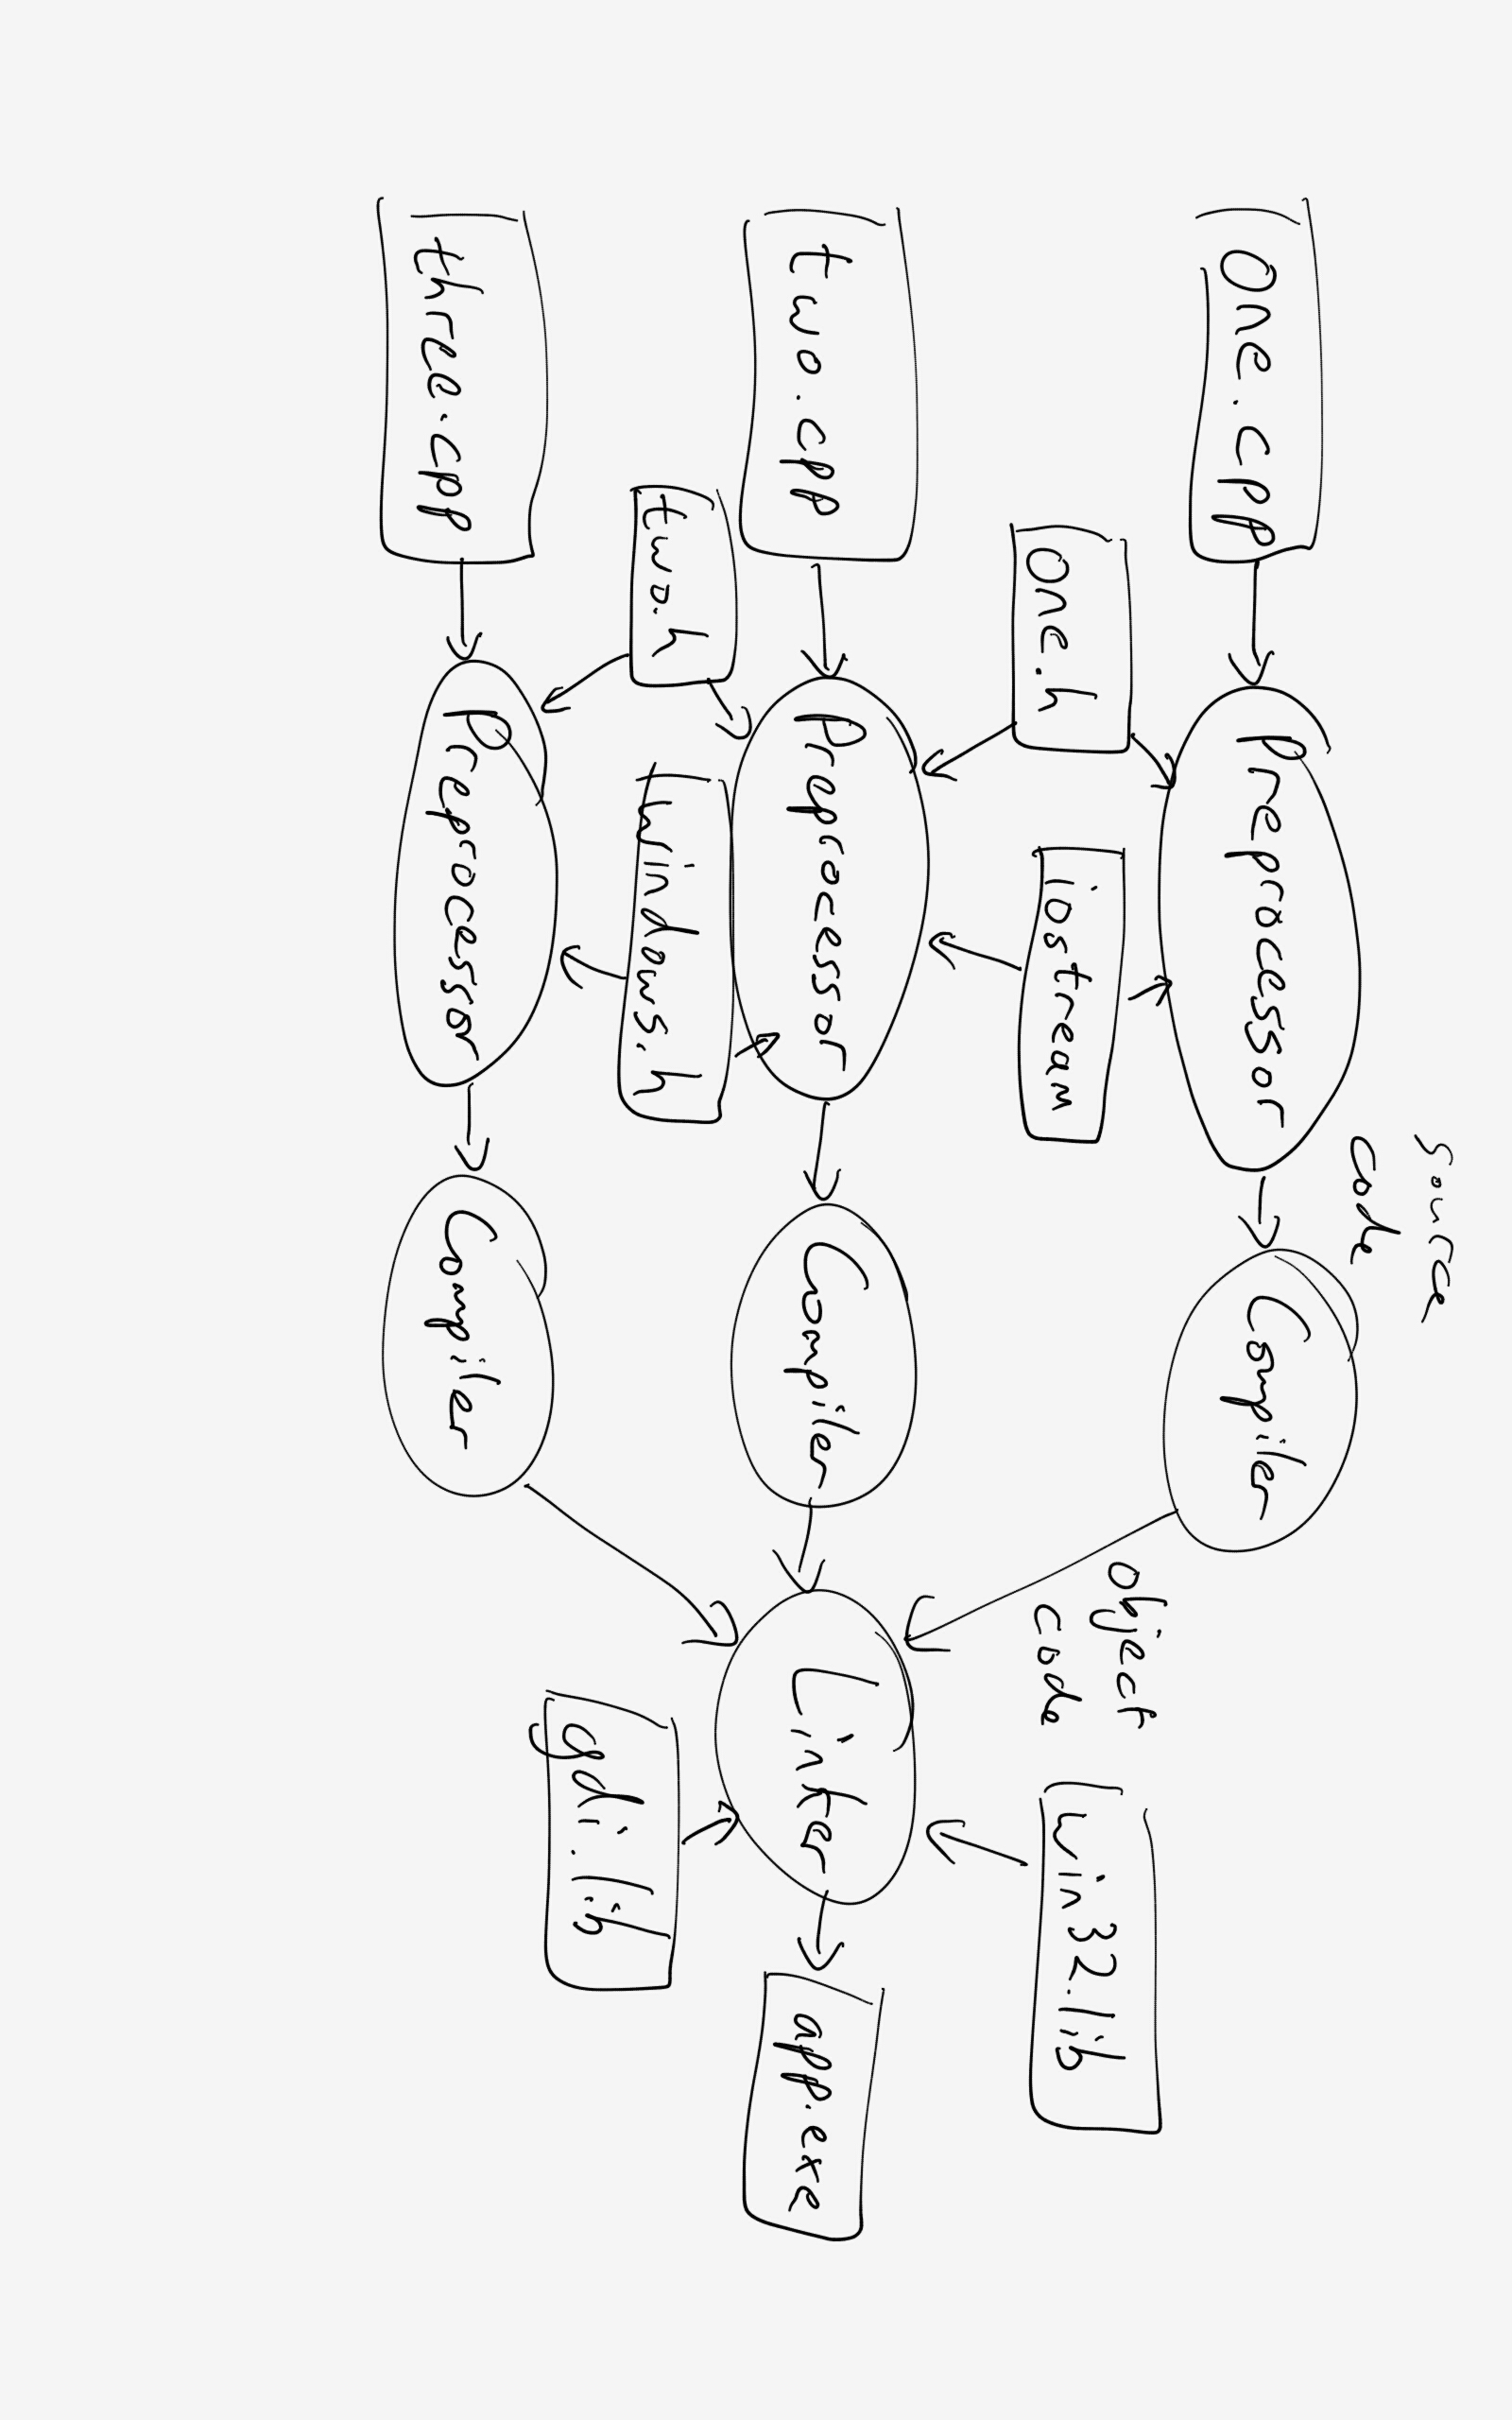
\includegraphics[height=\textwidth,angle=90]{compiler_sketch}
%\end{frame}

\end{document}
